

%----------------------------------------------------------------------------------------
%	PACKAGES AND OTHER DOCUMENT CONFIGURATIONS
%----------------------------------------------------------------------------------------

\documentclass[12pt]{article}
 
\usepackage{polski}
\usepackage[polish]{babel}
\usepackage[utf8]{inputenc}
\usepackage{datetime}
\usepackage{graphicx}
\usepackage{tikz} 
\usepackage{amsmath}
\usepackage{epstopdf}
\usepackage{array,booktabs}
\usepackage{float}
%\usepackage[colorlinks=true]{hyperref}
%\usepackage[all]{hypcap}
%\usepackage{showframe}
\usepackage{geometry}
 \geometry{
 a4paper, 
 left=30mm,
 right=30mm,
 top=30mm,
 bottom=30mm,
 }
 
\newdate{create_date}{19}{05}{2014}

%----------------------------------------------------------------------------------------

%----------------------------------------------------------------------------------------
% TIKZ PACKAGES
%----------------------------------------------------------------------------------------

\usetikzlibrary{arrows, calc}

%----------------------------------------------------------------------------------------

\begin{document}

\begin{titlepage}

\newcommand{\HRule}{\rule{\linewidth}{0.5mm}}
% Defines a new command for the horizontal lines, change thickness here

\center
% Center everything on the page
 
%----------------------------------------------------------------------------------------
%	LOGO SECTION
%----------------------------------------------------------------------------------------


\includegraphics[width=6cm]{../res/img/logo.png}\\[1cm]
% Include a department/university logo - this will require the graphicx package
 
%----------------------------------------------------------------------------------------
 
%----------------------------------------------------------------------------------------
%	HEADING SECTIONS
%----------------------------------------------------------------------------------------

\textsc{\LARGE Akademia Górniczo-Hutnicza \\[0.2cm]
im. Stanisława Staszica w Krakowie}\\[1.5cm]
% Name of your university/college

\textsc{\Large Podstawy Automatyki}\\[0.5cm]
% Major heading such as course name

%----------------------------------------------------------------------------------------
%	TITLE SECTION
%----------------------------------------------------------------------------------------

\HRule \\[0.5cm]
{ \huge \bfseries Dyskretne układy regulacji \\[0.3cm] oraz \\[0.5cm] Analiza
serwomechanizmu \\[0.2cm] przekaźnikowego z wykorzystaniem płaszczyzny
fazowej}\\[0.3cm]
% Title of your document
\HRule \\[1.5cm]
 
%----------------------------------------------------------------------------------------
%	AUTHOR SECTION
%----------------------------------------------------------------------------------------

% \begin{minipage}{0.4\textwidth}
% \begin{flushleft} \large
% \emph{Author:}\\
% Konrad \textsc{Adasiewcz} % Your name
% \end{flushleft}
% \end{minipage}
% ~
% \begin{minipage}{0.4\textwidth}
% \begin{flushright} \large
% \emph{Supervisor:} \\
% dr inż. Paweł \textsc{Rotter} % Supervisor's Name
% \end{flushright}
% \end{minipage}\\[4cm]

% If you don't want a supervisor, uncomment the two lines below and remove the section above
\flushright
\Large \emph{Autorzy:}\\
Konrad \textsc{Adasiewcz}\\[0.1cm] % Your name
Michał \textsc{Maciejewski}\\[3cm] % Your name

%----------------------------------------------------------------------------------------
%	DATE SECTION
%----------------------------------------------------------------------------------------
Data wykonania ćwiczenia: \\
{\large \displaydate{exercise_date}}\\[1cm]


\vfill % Fill the rest of the page with whitespace

\end{titlepage}

\section{Wstęp}

\subsection{Cel ćwiczenia}

Celem ćwiczenia jest identyfikacja parametrów modelu rzeczywistego obiektu regulacji. Obiekt 
rzeczywisty jest obiektem nieskończenie wymiarowym, ale dla celów sterowania może być opisany 
poniższymi modelami transmitancyjnymi Kupfmuellera I i II rzędu z opóźnieniem,
oraz modelem Strejca $n$-tego rzędu bez opóźnienia:

\begin{equation}
	G(s)=\dfrac{ke^{-s\tau}}{sT+1}
	\label{equ:trankup1}
\end{equation}

\begin{equation}
	G(s)=\frac{ke^{-s\tau}}{(T_1s+1)(T_2s+1)}
	\label{equ:trankup2}
\end{equation}

\begin{equation}
	G(s)=\frac{k}{(sT+1)^n}
	\label{equ:transtrejc}
\end{equation}

\newpage

\section{Model Kupfmuellera I rzędu z opóźnieniem}

Model Kupfmuellera I rzędu z opóźnieniem jest najprostszym ideowo modelem którym jesteśmy
w stanie z dość przyzwoitą dokładnością przybliżać wiele rodzajów obiektów rzeczywistych.

\begin{figure}[!htb]
	\begin{center}
		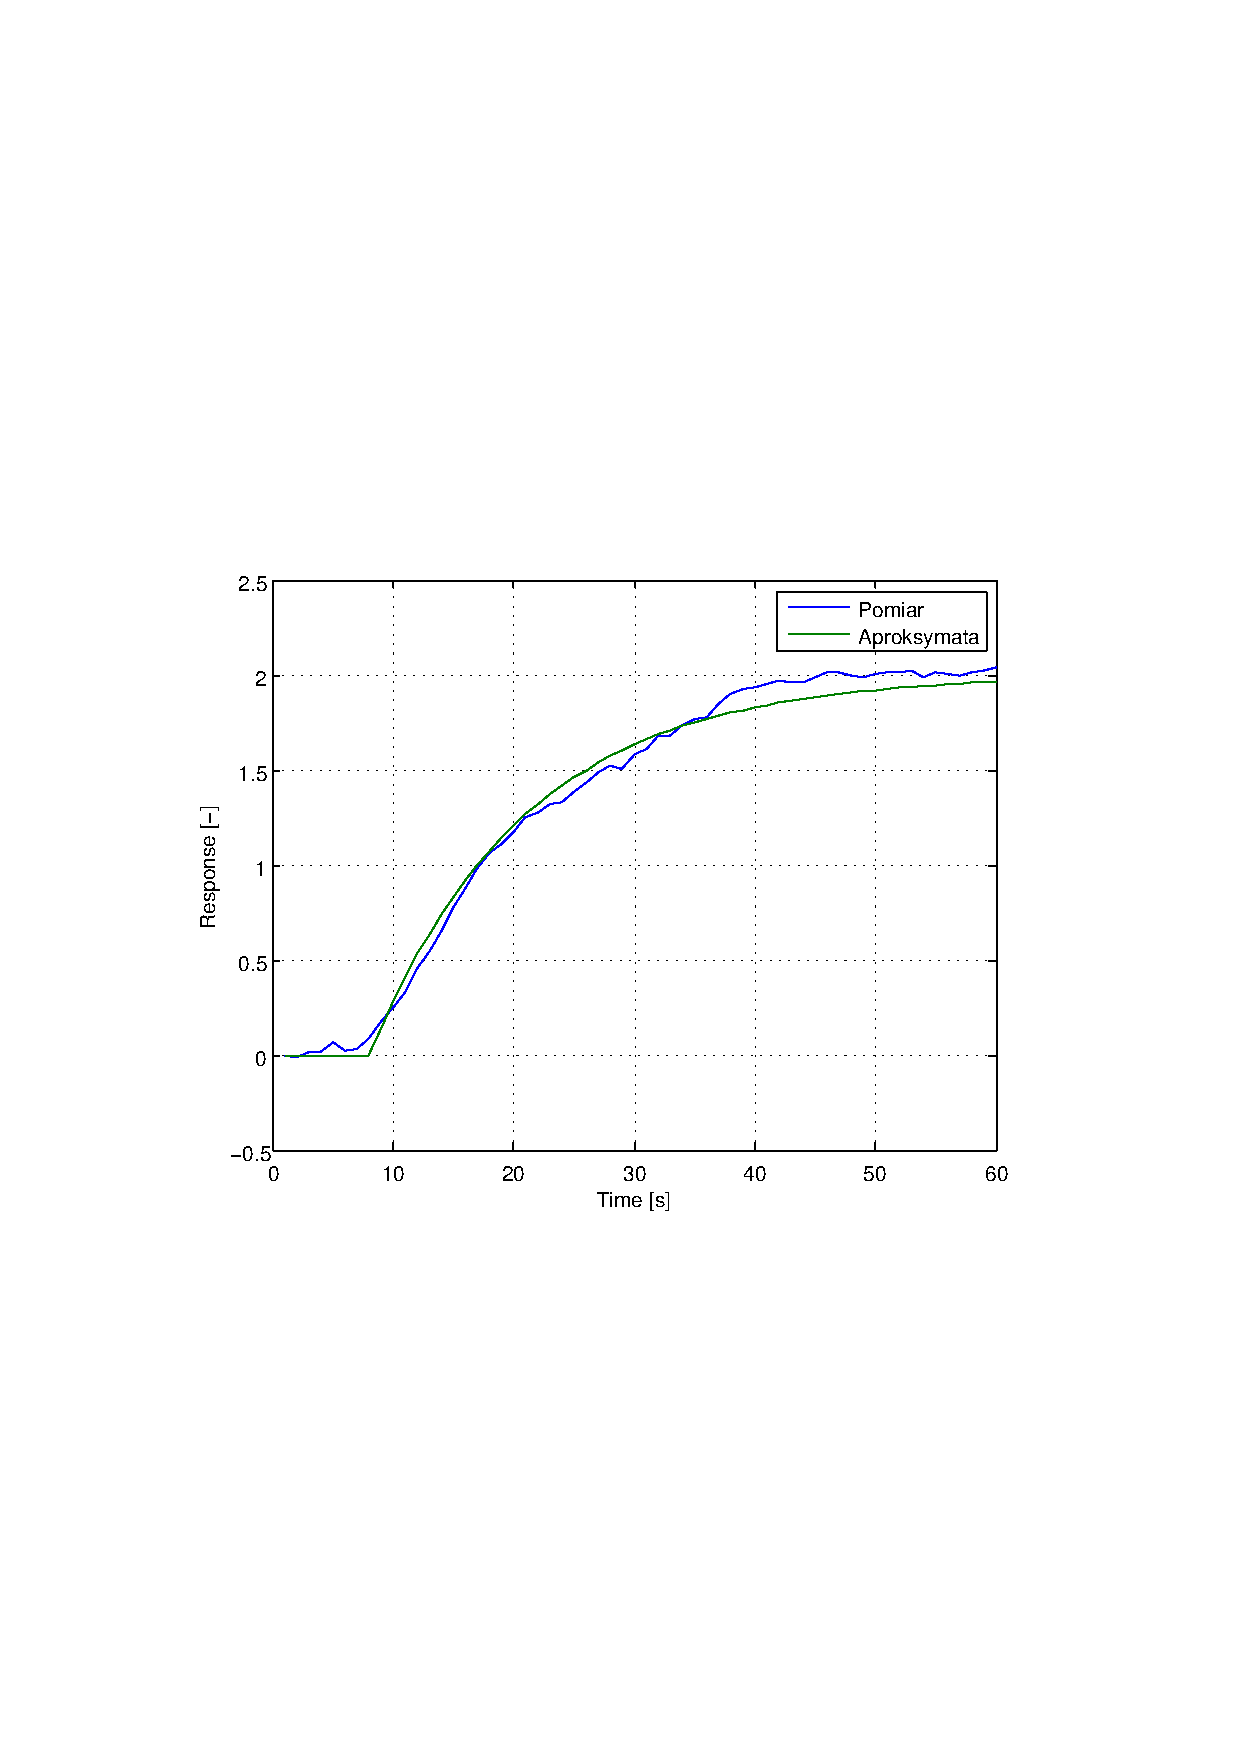
\includegraphics[width=14cm,trim=3cm 9cm 3cm 9cm,clip]
		{../res/img/k1_2_13_8.pdf}
	\end{center}
	\caption{Odpowiedź skokowa modelu na tle pomiarów dla parametrów modelu:
	$k=2[-]$, $T=13[s]$, $\theta=8[s]$. $\varepsilon=0.0046$}
\end{figure}

Pierwszym podejściem do odnalezienia parametrów modelu jest empiryczne
przybliżenie odpowiedzi skokowych poprzez ręczną zmianę parametrów na wyczucie.

Model minimalny względem całki z kwadratu błędu został wyznaczony przy pomocy
funkcji Matlabowskiej \textit{fminsearch}. Otrzymane parametry optymalne to:
$k=2.15[-]$, $T=15.8[s]$, $\theta=7.9[s]$.

\newpage

\begin{figure}[!htb]
	\begin{center}
		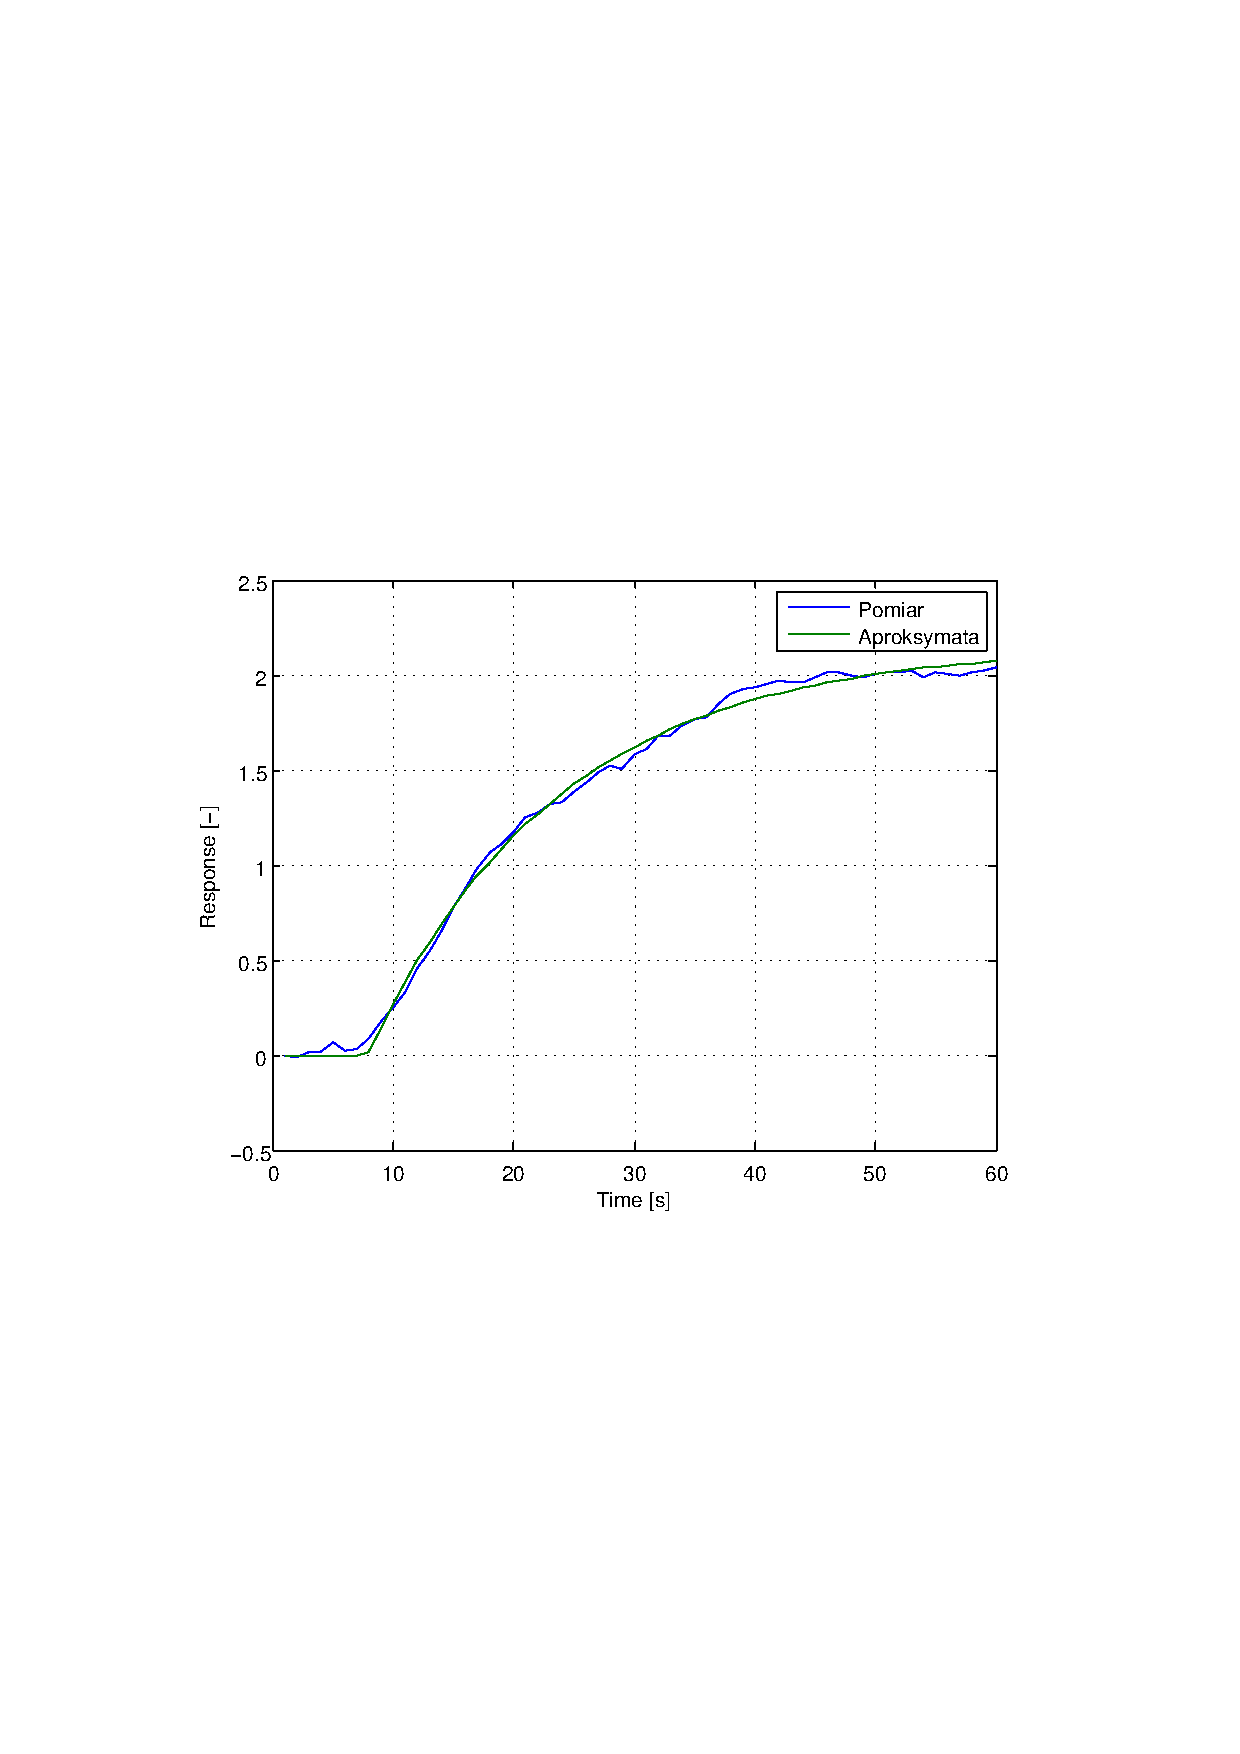
\includegraphics[width=14cm,trim=3cm 9cm 3cm 9cm,clip]
		{../res/img/k1_opt.pdf}
	\end{center}
	\caption{Odpowiedź skokowa modelu na tle pomiarów dla optymalnych parametrów
	modelu. $\varepsilon=0.0015$}
\end{figure}

\newpage

\subsection{Model Kupfmuellera II rzędu z opóźnieniem}

\begin{figure}[!htb]
	\begin{center}
		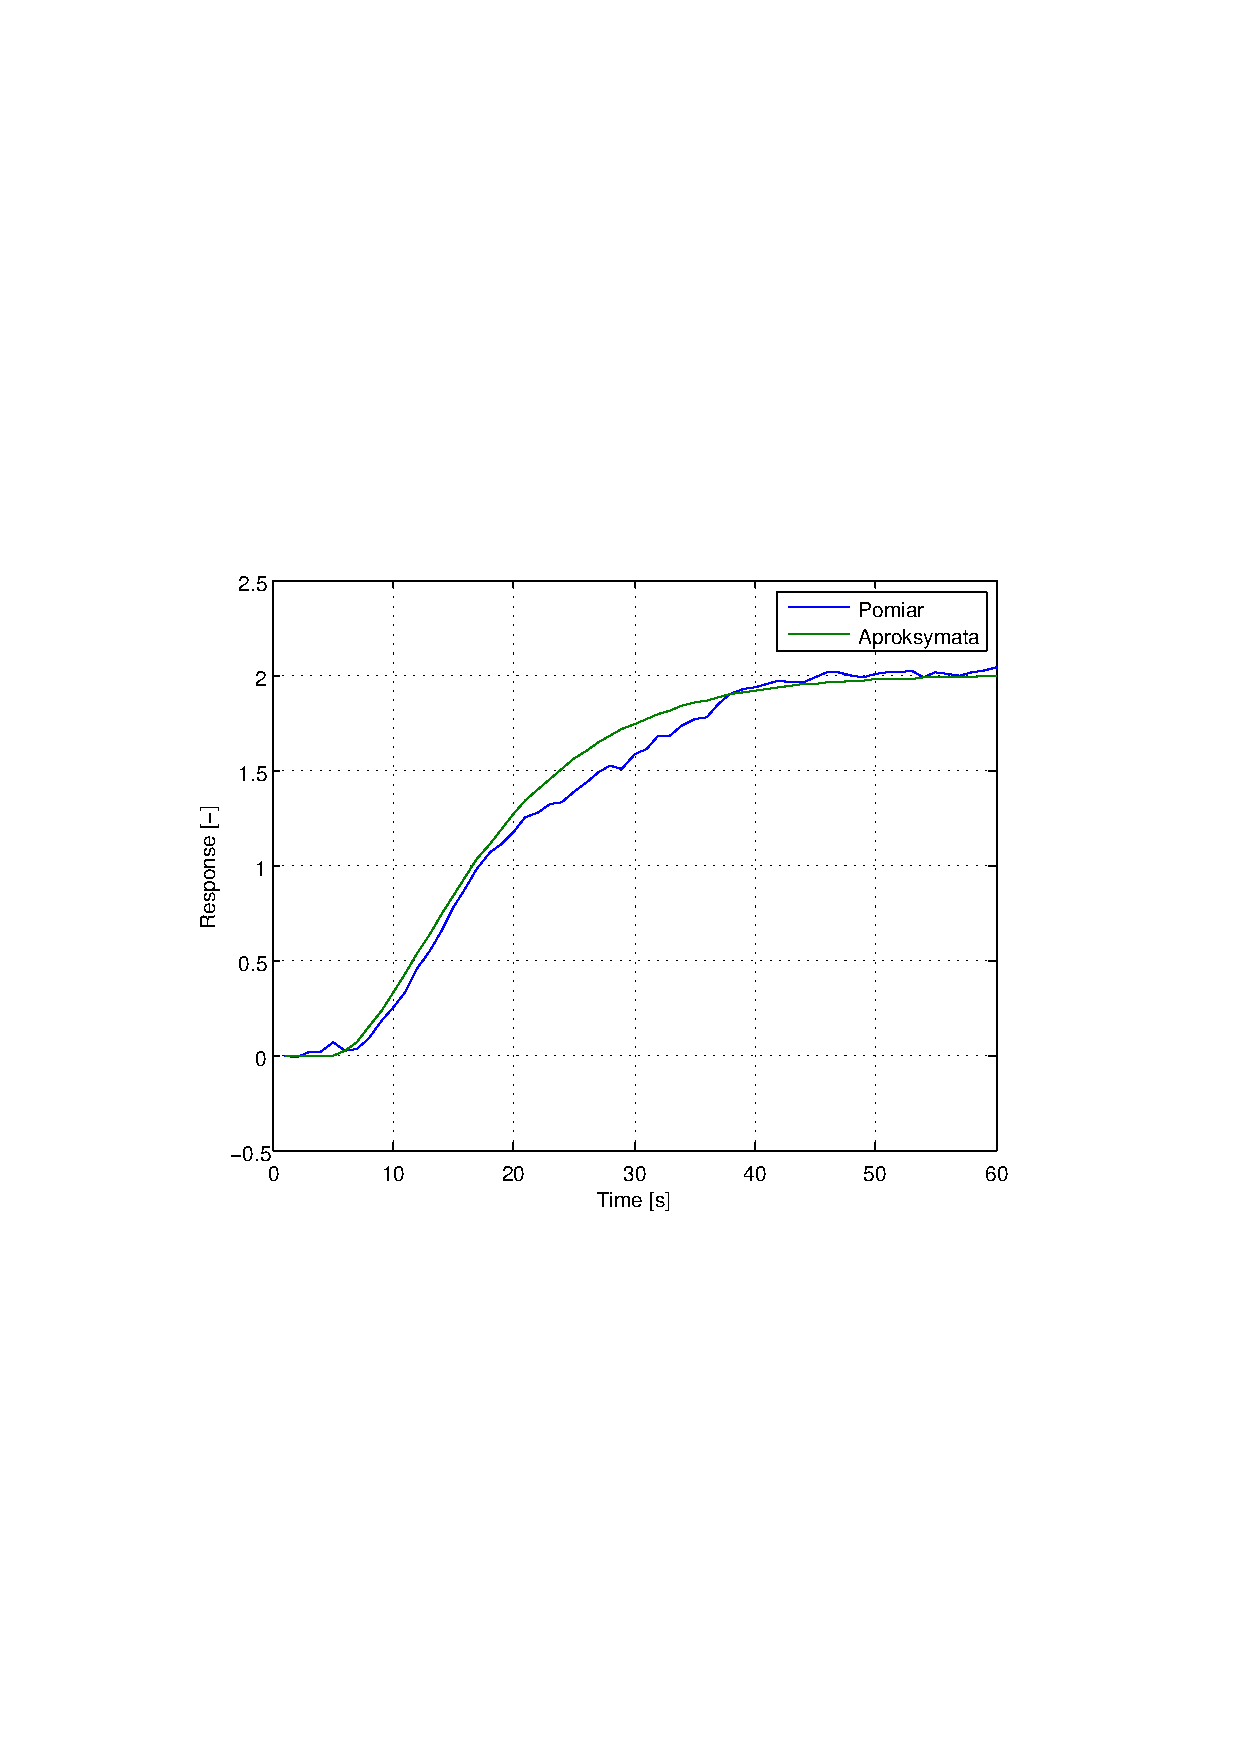
\includegraphics[width=14cm,trim=3cm 9cm 3cm 9cm,clip]
		{../res/img/k2_2_6_8_5.pdf}
	\end{center}
	\caption{Odpowiedź skokowa modelu na tle pomiarów dla parametrów modelu:
	$k=2[-]$, $T_1=6[s]$, $T_2=8[s]$, $\theta=5[s]$. $\varepsilon=0.0071$}
\end{figure}

Parametry dobrane empirycznie dają model odpowiadający skokowo jak na powyższej
charakterystyce.

\newpage

\begin{figure}[!htb]
	\begin{center}
		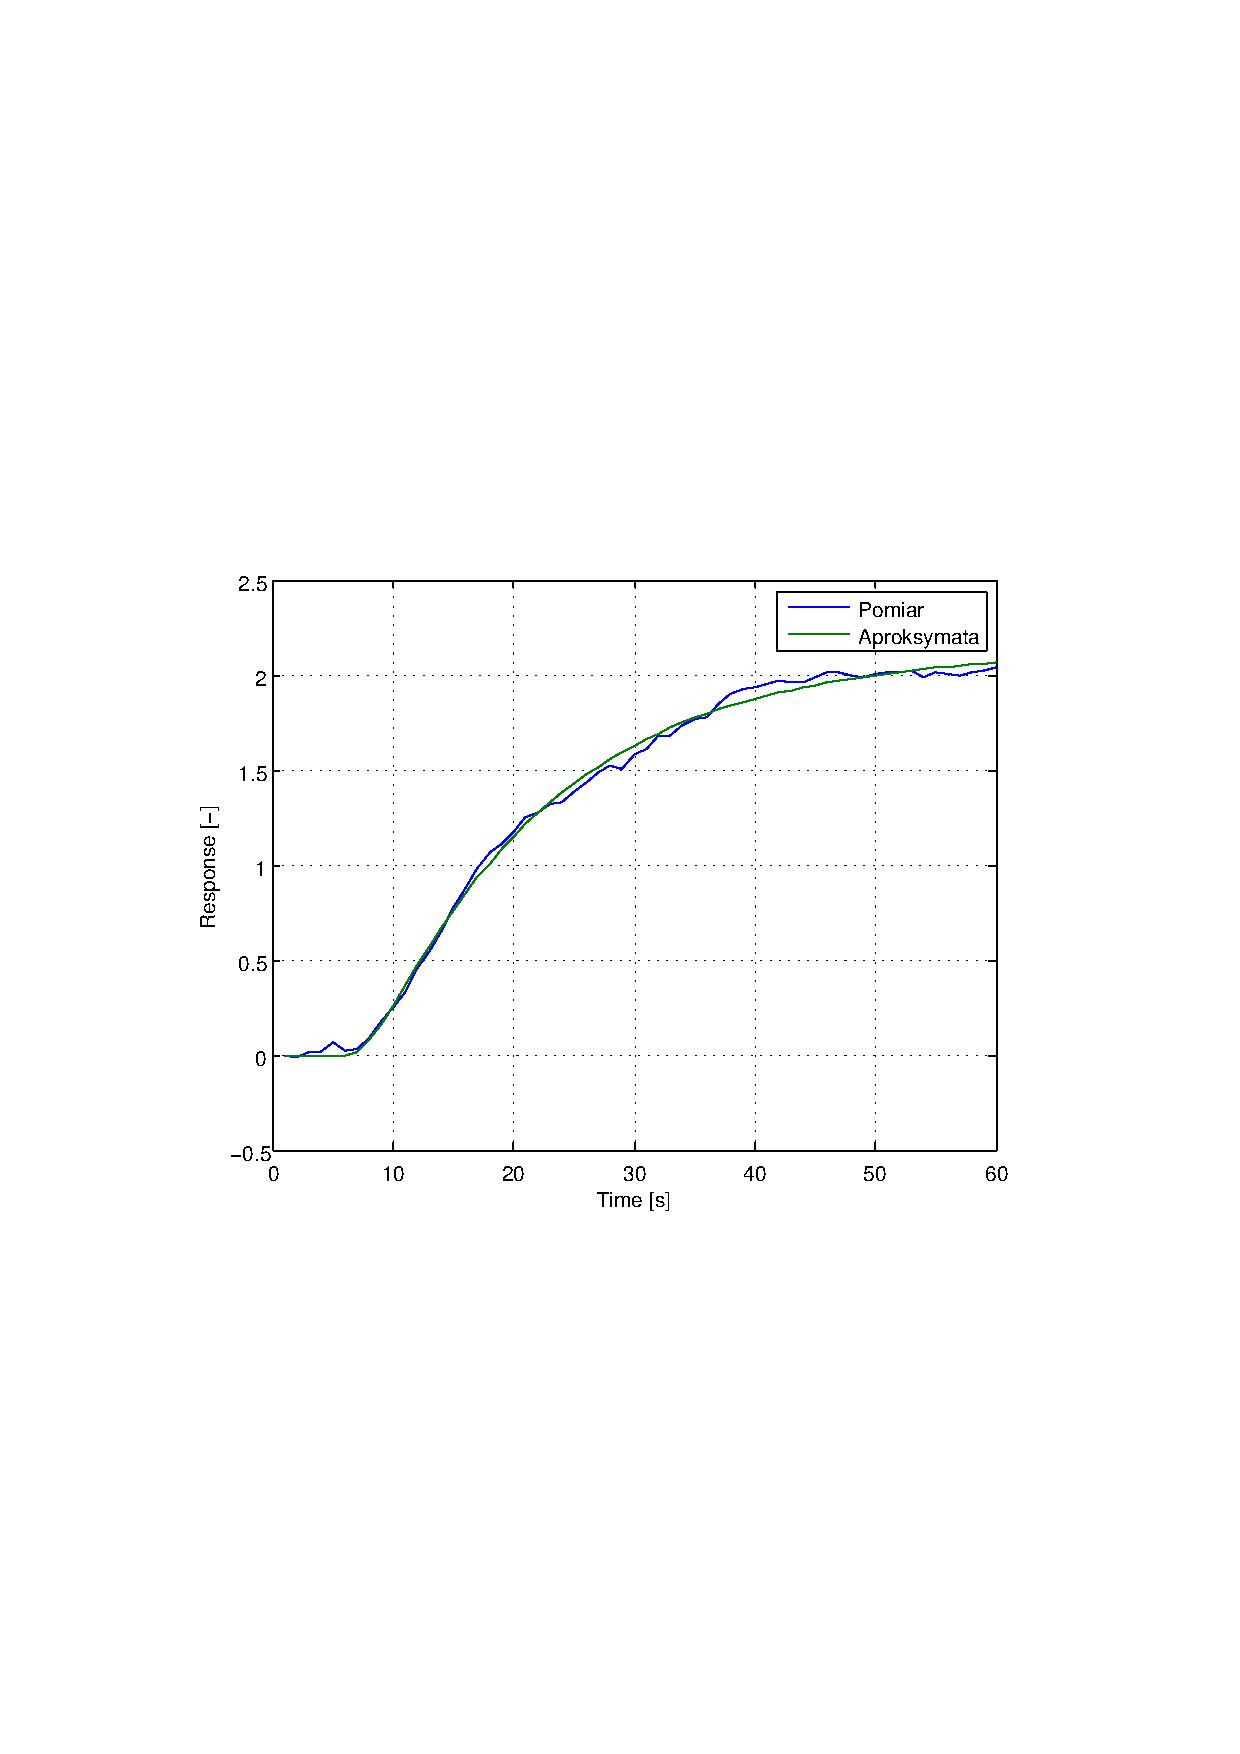
\includegraphics[width=14cm,trim=3cm 9cm 3cm 9cm,clip]
		{../res/img/k2_opt.pdf}
	\end{center}
	\caption{Odpowiedź skokowa modelu na tle pomiarów dla optymalnych parametrów
	modelu. $\varepsilon=0.0013$}
\end{figure}

Model optymalny ze względu na całkę z kwadratu błędu jest dokładniejszy niż
model pierwszego rzędu. Otrzymane parametry optymalne to:
$k=2.13[-]$, $T_1=14.84[s]$, $T_2=2.05[s]$, $\theta=6.28[s]$.

\newpage

\subsection{Model Strejca}

\begin{figure}[!htb]
	\begin{center}
		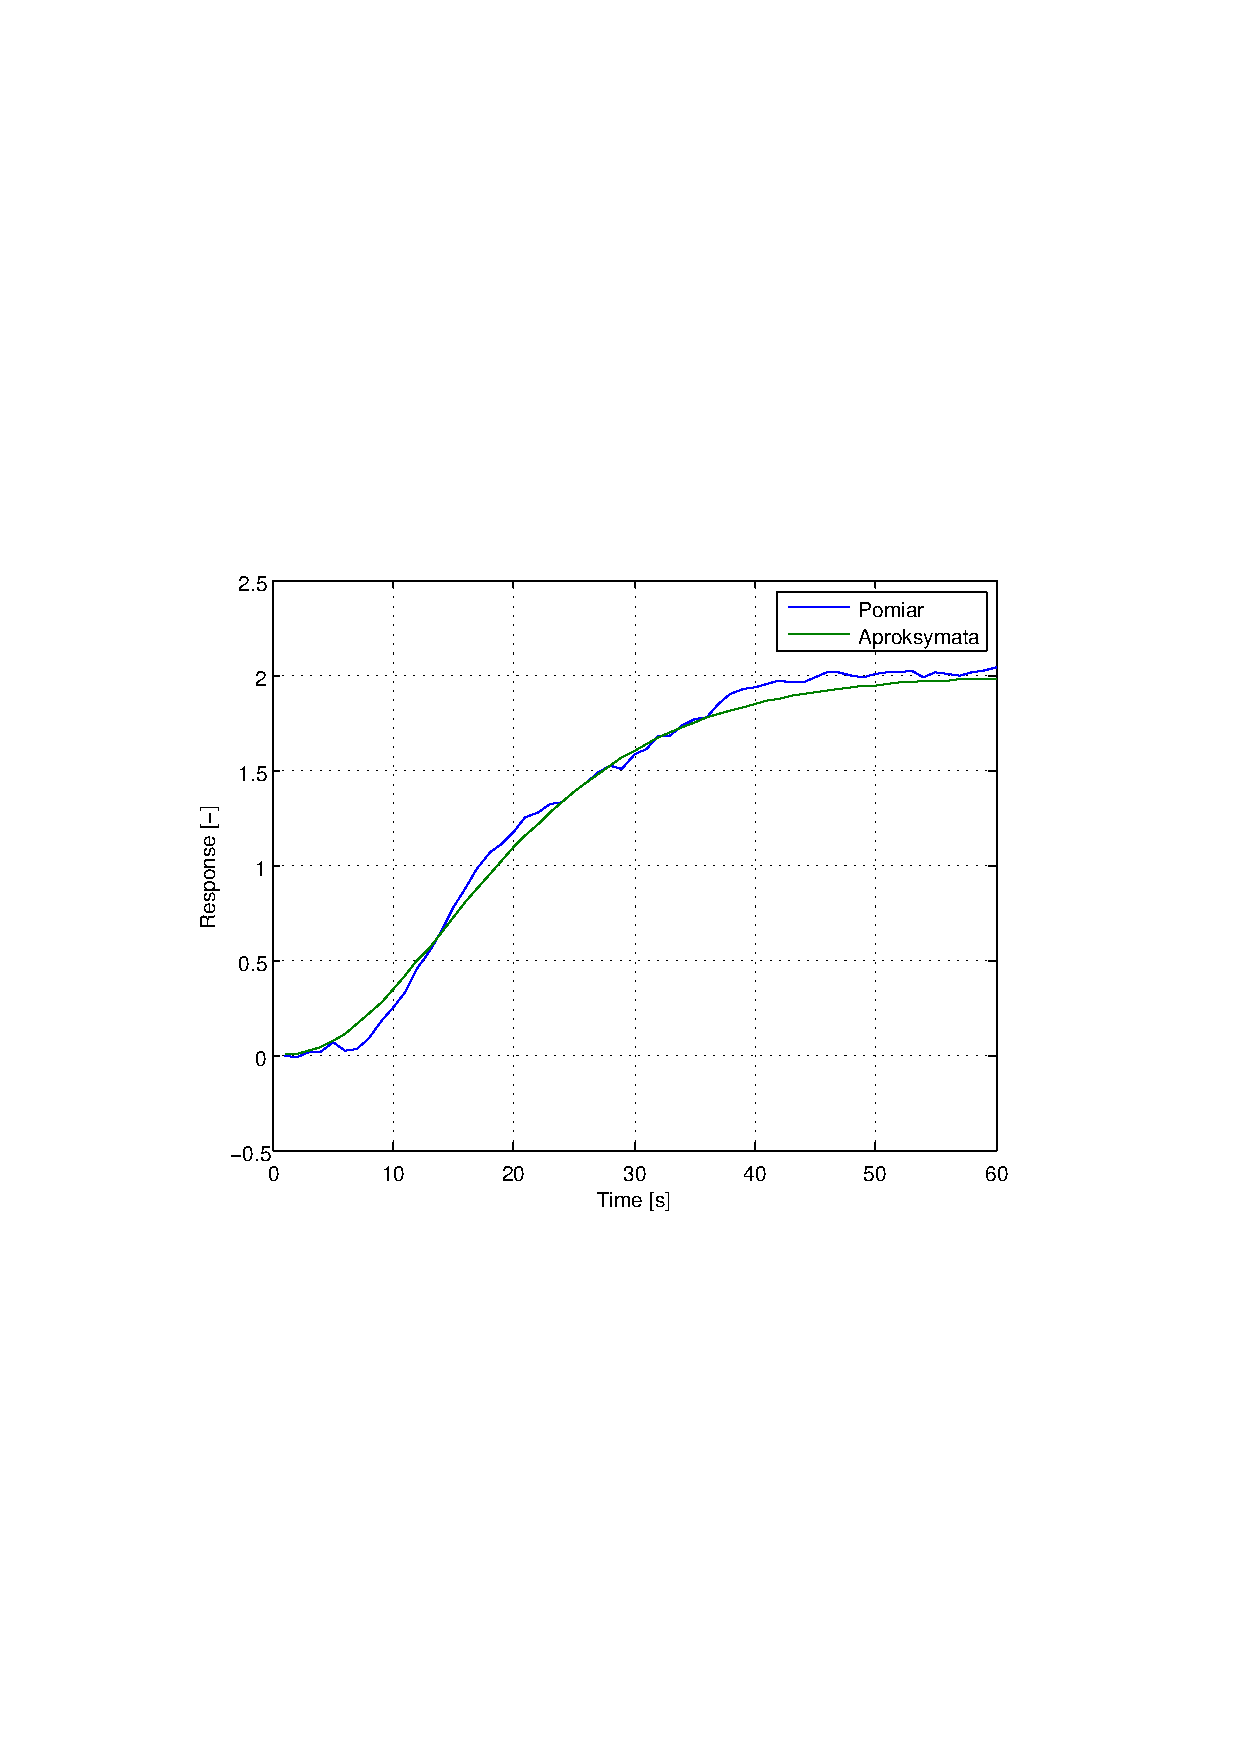
\includegraphics[width=14cm,trim=3cm 9cm 3cm 9cm,clip]
		{../res/img/k3_2_7_3.pdf}
	\end{center}
	\caption{Odpowiedź skokowa modelu na tle pomiarów dla parametrów modelu:
	$k=2[-]$, $T=7[s]$, $n=3[-]$. $\varepsilon=0.0041$}
\end{figure}

Ręczny dobór parametrów doprowadził mnie do powyższego modelu.

\newpage 

\begin{figure}[!htb]
	\begin{center}
		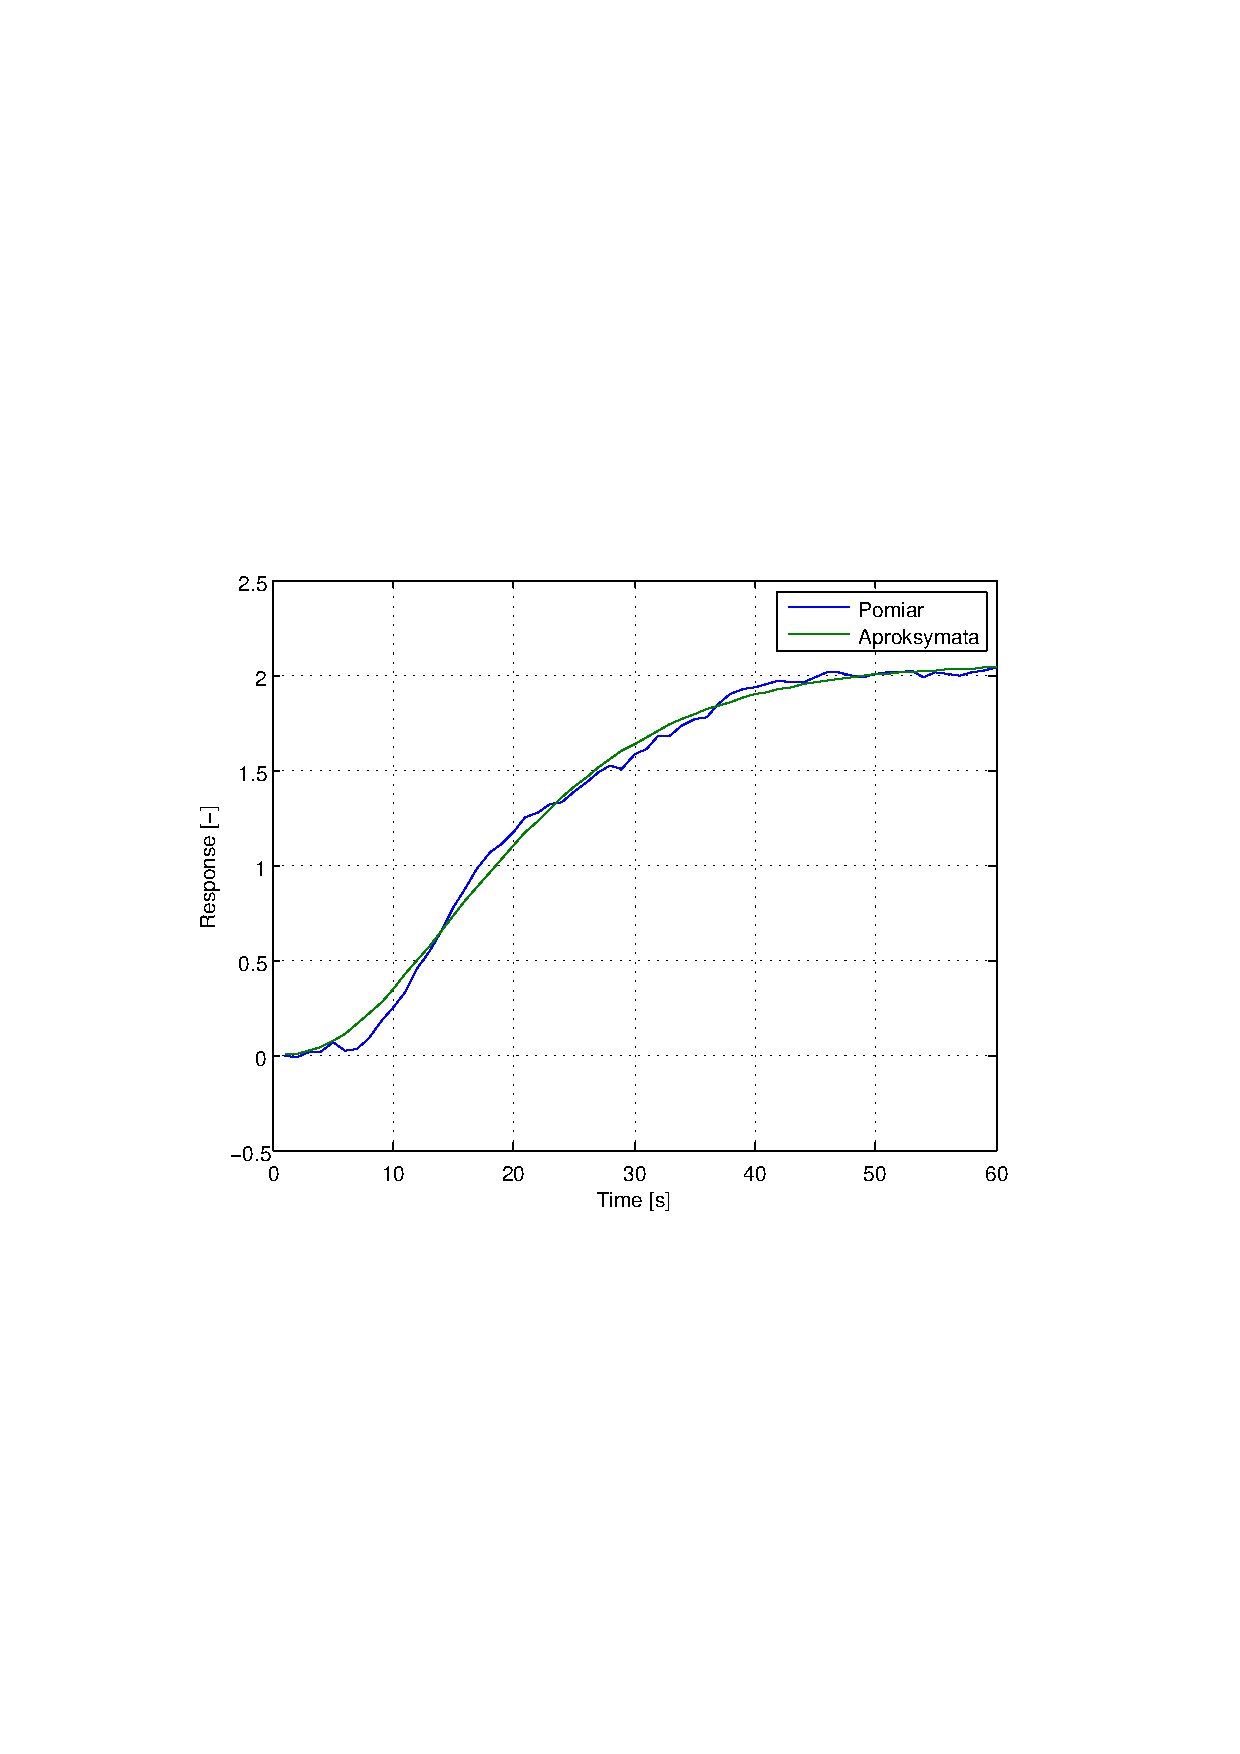
\includegraphics[width=14cm,trim=3cm 9cm 3cm 9cm,clip]
		{../res/img/k3_opt_3.pdf}
	\end{center}
	\caption{Odpowiedź skokowa modelu na tle pomiarów dla optymalnych parametrów
	modelu i rzędu aproksymacji $n=3[-]$. $\varepsilon=0.0027$}
\end{figure}

Parametry optymalne: $k=2.06[-]$, $T=7.08[s]$, $n=3[-]$.


\newpage

\section{Wnioski i spostrzeżenia}

Rzeczywiste obiekty dynamiczne są obiektami wysokich rzędów, można jednak
przybliżać je modelami niższych rzędów sprowadzając różnicę odpowiedzi skokowych
do minimum.

Modelem, którego odpowiedź najbardziej przypominała odpowiedź badanego obiektu był
model Kupfmuellera II rzędu z opóźnieniem, co nie jest zadziwiające, ponieważ jest on modelem
najbardziej swobodnym z badanych(kształt odpowiedzi zależał aż od czterech
zmiennych ciągłych).
Warto zauważyć, że pomimo iż model Strejca choć okazał się być najgorszym przybliżeniem
badanego obiektu, jest bardzo wygodny w analizie, ponieważ jego transmitancja wyrażona jest
skończonym ułamkiem wymiernym. Istotną cechą tego modelu jest również to, iż przestrzeń
możliwych do wybrania parametrów dla tego modelu jest najwęższa, ponieważ jeden z pa-
rametrów wyrażony jest liczbą naturalną, co powoduje iż jest on często wykorzystywany do
automatycznej identyfikacji obiektów.
 

\end{document}